\documentclass[]{article}
\usepackage{lmodern}
\usepackage{amssymb,amsmath}
\usepackage{ifxetex,ifluatex}
\usepackage{fixltx2e} % provides \textsubscript
\ifnum 0\ifxetex 1\fi\ifluatex 1\fi=0 % if pdftex
  \usepackage[T1]{fontenc}
  \usepackage[utf8]{inputenc}
\else % if luatex or xelatex
  \ifxetex
    \usepackage{mathspec}
  \else
    \usepackage{fontspec}
  \fi
  \defaultfontfeatures{Ligatures=TeX,Scale=MatchLowercase}
\fi
% use upquote if available, for straight quotes in verbatim environments
\IfFileExists{upquote.sty}{\usepackage{upquote}}{}
% use microtype if available
\IfFileExists{microtype.sty}{%
\usepackage{microtype}
\UseMicrotypeSet[protrusion]{basicmath} % disable protrusion for tt fonts
}{}
\usepackage[margin=1in]{geometry}
\usepackage{hyperref}
\hypersetup{unicode=true,
            pdfauthor={Knitted by Forename Surname on 12 December 2019},
            pdfborder={0 0 0},
            breaklinks=true}
\urlstyle{same}  % don't use monospace font for urls
\usepackage{color}
\usepackage{fancyvrb}
\newcommand{\VerbBar}{|}
\newcommand{\VERB}{\Verb[commandchars=\\\{\}]}
\DefineVerbatimEnvironment{Highlighting}{Verbatim}{commandchars=\\\{\}}
% Add ',fontsize=\small' for more characters per line
\usepackage{framed}
\definecolor{shadecolor}{RGB}{248,248,248}
\newenvironment{Shaded}{\begin{snugshade}}{\end{snugshade}}
\newcommand{\AlertTok}[1]{\textcolor[rgb]{0.94,0.16,0.16}{#1}}
\newcommand{\AnnotationTok}[1]{\textcolor[rgb]{0.56,0.35,0.01}{\textbf{\textit{#1}}}}
\newcommand{\AttributeTok}[1]{\textcolor[rgb]{0.77,0.63,0.00}{#1}}
\newcommand{\BaseNTok}[1]{\textcolor[rgb]{0.00,0.00,0.81}{#1}}
\newcommand{\BuiltInTok}[1]{#1}
\newcommand{\CharTok}[1]{\textcolor[rgb]{0.31,0.60,0.02}{#1}}
\newcommand{\CommentTok}[1]{\textcolor[rgb]{0.56,0.35,0.01}{\textit{#1}}}
\newcommand{\CommentVarTok}[1]{\textcolor[rgb]{0.56,0.35,0.01}{\textbf{\textit{#1}}}}
\newcommand{\ConstantTok}[1]{\textcolor[rgb]{0.00,0.00,0.00}{#1}}
\newcommand{\ControlFlowTok}[1]{\textcolor[rgb]{0.13,0.29,0.53}{\textbf{#1}}}
\newcommand{\DataTypeTok}[1]{\textcolor[rgb]{0.13,0.29,0.53}{#1}}
\newcommand{\DecValTok}[1]{\textcolor[rgb]{0.00,0.00,0.81}{#1}}
\newcommand{\DocumentationTok}[1]{\textcolor[rgb]{0.56,0.35,0.01}{\textbf{\textit{#1}}}}
\newcommand{\ErrorTok}[1]{\textcolor[rgb]{0.64,0.00,0.00}{\textbf{#1}}}
\newcommand{\ExtensionTok}[1]{#1}
\newcommand{\FloatTok}[1]{\textcolor[rgb]{0.00,0.00,0.81}{#1}}
\newcommand{\FunctionTok}[1]{\textcolor[rgb]{0.00,0.00,0.00}{#1}}
\newcommand{\ImportTok}[1]{#1}
\newcommand{\InformationTok}[1]{\textcolor[rgb]{0.56,0.35,0.01}{\textbf{\textit{#1}}}}
\newcommand{\KeywordTok}[1]{\textcolor[rgb]{0.13,0.29,0.53}{\textbf{#1}}}
\newcommand{\NormalTok}[1]{#1}
\newcommand{\OperatorTok}[1]{\textcolor[rgb]{0.81,0.36,0.00}{\textbf{#1}}}
\newcommand{\OtherTok}[1]{\textcolor[rgb]{0.56,0.35,0.01}{#1}}
\newcommand{\PreprocessorTok}[1]{\textcolor[rgb]{0.56,0.35,0.01}{\textit{#1}}}
\newcommand{\RegionMarkerTok}[1]{#1}
\newcommand{\SpecialCharTok}[1]{\textcolor[rgb]{0.00,0.00,0.00}{#1}}
\newcommand{\SpecialStringTok}[1]{\textcolor[rgb]{0.31,0.60,0.02}{#1}}
\newcommand{\StringTok}[1]{\textcolor[rgb]{0.31,0.60,0.02}{#1}}
\newcommand{\VariableTok}[1]{\textcolor[rgb]{0.00,0.00,0.00}{#1}}
\newcommand{\VerbatimStringTok}[1]{\textcolor[rgb]{0.31,0.60,0.02}{#1}}
\newcommand{\WarningTok}[1]{\textcolor[rgb]{0.56,0.35,0.01}{\textbf{\textit{#1}}}}
\usepackage{graphicx,grffile}
\makeatletter
\def\maxwidth{\ifdim\Gin@nat@width>\linewidth\linewidth\else\Gin@nat@width\fi}
\def\maxheight{\ifdim\Gin@nat@height>\textheight\textheight\else\Gin@nat@height\fi}
\makeatother
% Scale images if necessary, so that they will not overflow the page
% margins by default, and it is still possible to overwrite the defaults
% using explicit options in \includegraphics[width, height, ...]{}
\setkeys{Gin}{width=\maxwidth,height=\maxheight,keepaspectratio}
\IfFileExists{parskip.sty}{%
\usepackage{parskip}
}{% else
\setlength{\parindent}{0pt}
\setlength{\parskip}{6pt plus 2pt minus 1pt}
}
\setlength{\emergencystretch}{3em}  % prevent overfull lines
\providecommand{\tightlist}{%
  \setlength{\itemsep}{0pt}\setlength{\parskip}{0pt}}
\setcounter{secnumdepth}{0}
% Redefines (sub)paragraphs to behave more like sections
\ifx\paragraph\undefined\else
\let\oldparagraph\paragraph
\renewcommand{\paragraph}[1]{\oldparagraph{#1}\mbox{}}
\fi
\ifx\subparagraph\undefined\else
\let\oldsubparagraph\subparagraph
\renewcommand{\subparagraph}[1]{\oldsubparagraph{#1}\mbox{}}
\fi

%%% Use protect on footnotes to avoid problems with footnotes in titles
\let\rmarkdownfootnote\footnote%
\def\footnote{\protect\rmarkdownfootnote}

%%% Change title format to be more compact
\usepackage{titling}

% Create subtitle command for use in maketitle
\providecommand{\subtitle}[1]{
  \posttitle{
    \begin{center}\large#1\end{center}
    }
}

\setlength{\droptitle}{-2em}

  \title{\#tilastoMOOC 2019--2020\\
\textbf{Helsinki Social Statistics}\\
Chapter 10. Regression}
    \pretitle{\vspace{\droptitle}\centering\huge}
  \posttitle{\par}
  \subtitle{\emph{Now, pick roles for the variables and start modeling. I predict
you are good!}}
  \author{Knitted by \textbf{Forename Surname} on 12 December 2019}
    \preauthor{\centering\large\emph}
  \postauthor{\par}
    \date{}
    \predate{}\postdate{}
  

\begin{document}
\maketitle

{
\setcounter{tocdepth}{2}
\tableofcontents
}
Chapter 10 consists of 7 exercises: 10.1 -- 10.7. Go to each exercise in
turn and do as follows:

\begin{enumerate}
\def\labelenumi{\arabic{enumi}.}
\tightlist
\item
  Read the brief description of the exercise.
\item
  Run the (possible) pre-exercise-code chunk.
\item
  Follow the instructions to fix the R code!
\end{enumerate}

General information on the MOOC platform (under Theme 1). Have fun!
\texttt{:-)}

\hypertarget{packages-in-r}{%
\subsection{10.1 Packages in R}\label{packages-in-r}}

Welcome to chapter 10: \textbf{Regression}. We'll start with an
important R feature - packages.

There are a lot of functions in R. But actually, the functions in R come
from a standard set of \emph{packages}. A package is simply a collection
of R functions. Besides the basic packages, you can install and use (or
develop!) other packages too.

You can install packages through CRAN (The Comprehensive R Archive
Network). From the CRAN website \url{https://cran.r-project.org/}:
\textgreater{} CRAN is a network of ftp and web servers around the world
that store identical, up-to-date, versions of code and documentation for
R.

List of available CRAN packages can be seen
\href{https://cran.r-project.org/web/packages/available_packages_by_name.html}{here}.
There are thousands of them, made by R users around the world. In order
to get a package accepted to CRAN, the package must be well documented:
every function must have a help page.

As you now have RStudio (and R) in your own computer, you can install R
packages anytime by calling
\texttt{install.packages("name\_of\_the\_package")}. This is best to be
done in the Console or in the Packages pane, where there is an Install
button.

To use installed packages, you need to access them. This is done by
calling \texttt{library(name\_of\_the\_package)}.

\hypertarget{instructions}{%
\subsubsection{Instructions}\label{instructions}}

\begin{itemize}
\tightlist
\item
  One of the most famous and used packages outside the basic R is
  \texttt{ggplot2}. The \texttt{ggplot2} package is a plotting system
  for R, and it draws pretty pictures for you with small effort.
\item
  The \texttt{ggplot2} package has a website \url{http://ggplot2.org/}
  where you can see documentation about the package.
\item
  Execute the access code for \texttt{ggplot2}.
\item
  Draw a plot of gender and points. The \texttt{fill} argument adds a
  legend to the plot.
\item
  Create the \texttt{grades} object.
\item
  Do a plot of \texttt{grades} and \texttt{attitude}. Set
  \texttt{grades} as a legend.
\end{itemize}

\hypertarget{r-code}{%
\subsubsection{R code}\label{r-code}}

\begin{Shaded}
\begin{Highlighting}[]
\CommentTok{# Work with the exercise in this chunk, step-by-step. Fix the R code!}

\CommentTok{# learning2014 is available }

\CommentTok{# Access ggplot2}
\KeywordTok{library}\NormalTok{(ggplot2)}

\CommentTok{# Draw a plot of gender and points}
\KeywordTok{qplot}\NormalTok{(gender, points, }\DataTypeTok{data=}\NormalTok{learning2014, }\DataTypeTok{geom=}\StringTok{"boxplot"}\NormalTok{, }\DataTypeTok{fill=}\NormalTok{gender)}
\end{Highlighting}
\end{Shaded}

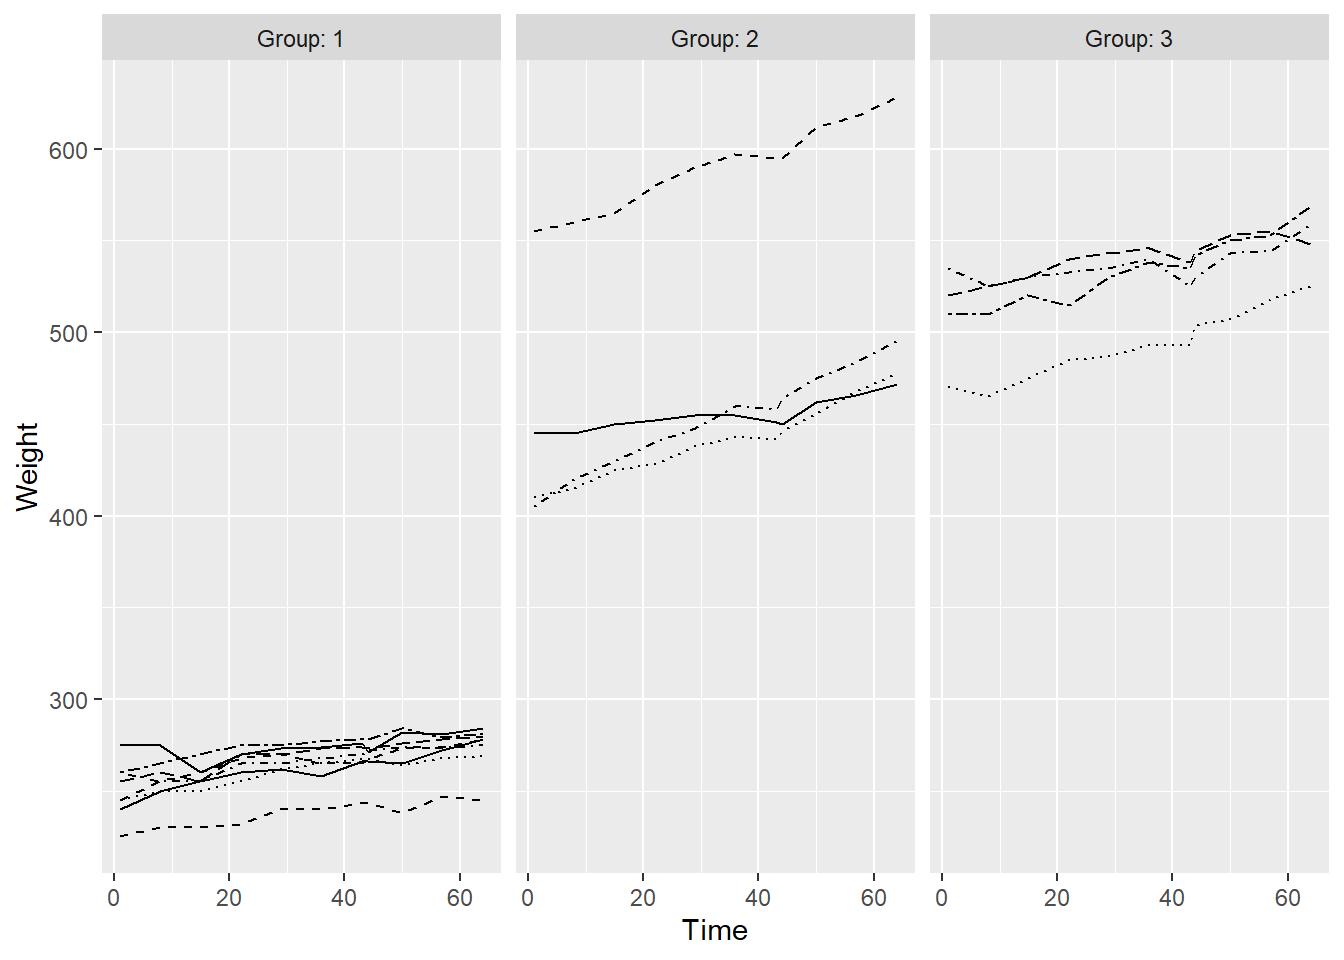
\includegraphics{jyt_chapter10_files/figure-latex/unnamed-chunk-2-1.pdf}

\begin{Shaded}
\begin{Highlighting}[]
\CommentTok{# Create the grades factor}
\NormalTok{grades <-}\StringTok{ }\KeywordTok{cut}\NormalTok{(learning2014}\OperatorTok{$}\NormalTok{points, }\DataTypeTok{breaks =} \KeywordTok{c}\NormalTok{(}\DecValTok{0}\NormalTok{, }\DecValTok{11}\NormalTok{, }\DecValTok{15}\NormalTok{, }\DecValTok{19}\NormalTok{, }\DecValTok{23}\NormalTok{, }\DecValTok{27}\NormalTok{, }\DecValTok{33}\NormalTok{), }\DataTypeTok{include.lowest =} \OtherTok{TRUE}\NormalTok{)}

\CommentTok{# Draw a plot of grades and attitude}
\CommentTok{#???}
\end{Highlighting}
\end{Shaded}

You have the keys do anything. Awesome!

\hypertarget{exploring-the-relationship-of-two-variables}{%
\subsection{10.2 Exploring the relationship of two
variables}\label{exploring-the-relationship-of-two-variables}}

It is always a good idea to start with the simplest possible
explorations before more complicated statistical analysis. A scatter
plot is always a good starting point when analyzing the relationship
between variables. Sample correlations are another useful tool.

In the ggplot2 library, scatter plots can be drawn with the general
\texttt{qplot()} function. \texttt{geom\_smooth()} can be used to add a
regression line to the plot. In base R \texttt{cor.test()} can be used
to compute a correlation with a confidence interval.

\hypertarget{instructions-1}{%
\subsubsection{Instructions}\label{instructions-1}}

\begin{itemize}
\tightlist
\item
  Access the ggplot2 library, modify the learning2014 data and draw a
  scatter plot of \texttt{attitude} and \texttt{points}.
\item
  Adjust the scatter plot: Add code \texttt{+\ geom\_smooth()} after
  \texttt{qplot()}. Write the code to the same line and do not forget
  the plus sign. Execute the row.
\item
  Give the function \texttt{geom\_smooth()} the argument
  \texttt{method\ =\ "lm"} and execute the line again. This adds a
  regression line along with a confidence interval.
\item
  Compute the correlation of \texttt{attitude} and \texttt{points} with
  \texttt{cor.test()}
\item
  Is a linear relationship between attitude and points plausible?
\item
  How would you characterize the strength of that relationship?
\end{itemize}

\hypertarget{r-code-1}{%
\subsubsection{R code}\label{r-code-1}}

\begin{Shaded}
\begin{Highlighting}[]
\CommentTok{# Work with the exercise in this chunk, step-by-step. Fix the R code!}

\CommentTok{# learning2014 is available}

\CommentTok{# Access ggplot2 functions}
\KeywordTok{library}\NormalTok{(ggplot2)}

\CommentTok{# Exlude students who did not attend any exams (points == 0)}
\NormalTok{learning2014 <-}\StringTok{ }\NormalTok{learning2014[learning2014}\OperatorTok{$}\NormalTok{points }\OperatorTok{!=}\StringTok{ }\DecValTok{0}\NormalTok{, ]}

\CommentTok{# Create objects attitude and points}
\NormalTok{attitude <-}\StringTok{ }\NormalTok{learning2014}\OperatorTok{$}\NormalTok{attitude}
\NormalTok{points <-}\StringTok{ }\NormalTok{learning2014}\OperatorTok{$}\NormalTok{points}

\CommentTok{# A scatter plot of attitude and points}
\KeywordTok{qplot}\NormalTok{(attitude, points) }\CommentTok{#???}
\end{Highlighting}
\end{Shaded}

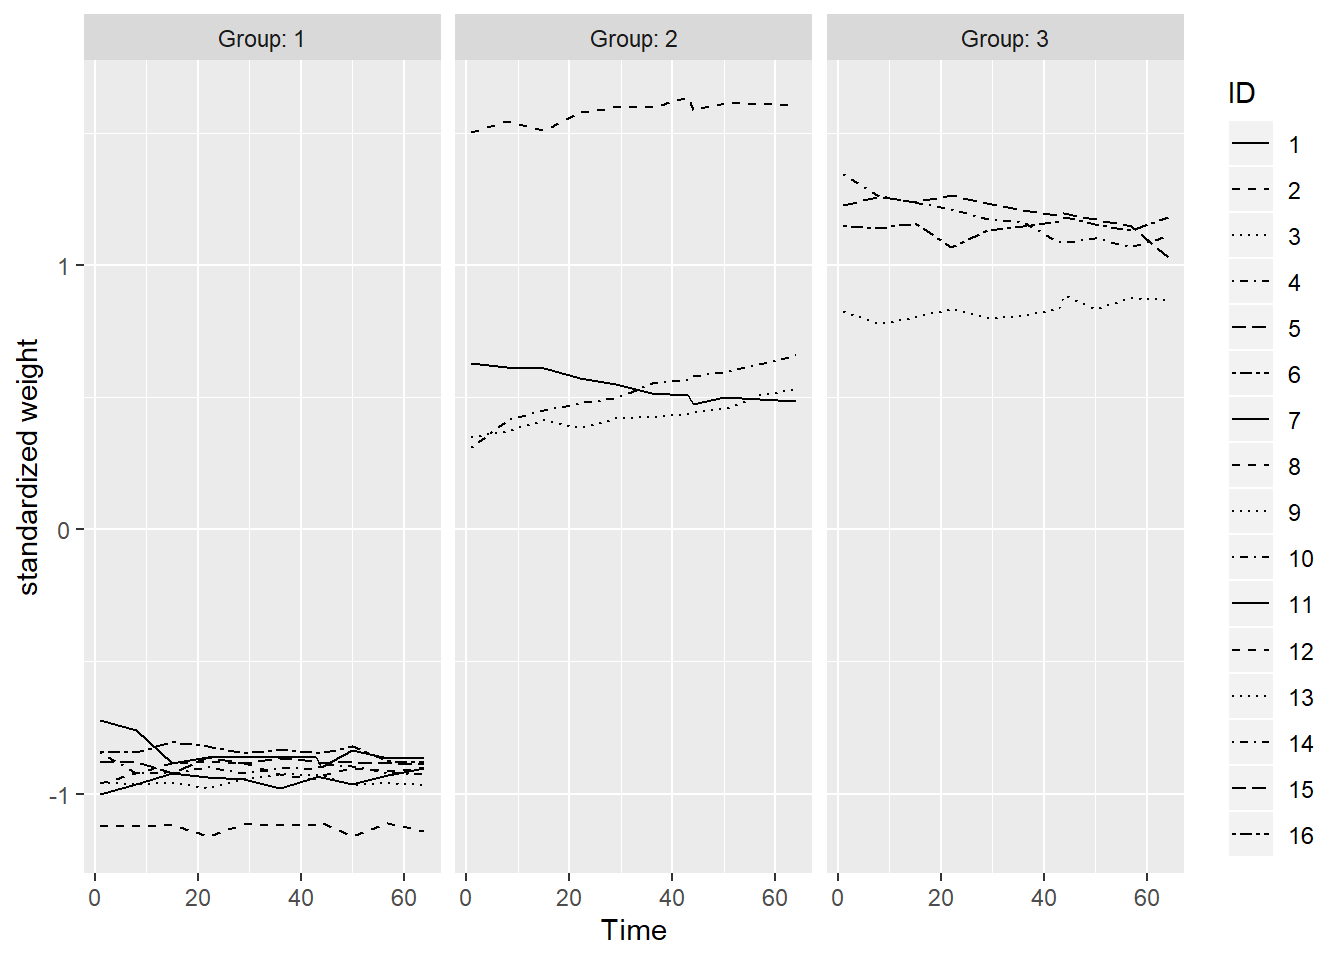
\includegraphics{jyt_chapter10_files/figure-latex/unnamed-chunk-4-1.pdf}

\begin{Shaded}
\begin{Highlighting}[]
\CommentTok{# Correlation with a confidence intervals}
\CommentTok{#???}
\end{Highlighting}
\end{Shaded}

\hypertarget{what-is-a-linear-model}{%
\subsection{10.3 What is a linear model?}\label{what-is-a-linear-model}}

Genrally, a
\href{https://en.wikipedia.org/wiki/Statistical_model}{statistical
model} embodies a set of assumptions concerning the generation of the
observed data and similar data from a larger population. A
\href{https://en.wikipedia.org/wiki/Linear_regression}{linear model}
makes the following assumptions:

\begin{itemize}
\tightlist
\item
  The mean of the response variable is a \emph{linear combination} of
  the explanatory variable(s) and the parameters.
\item
  The prediction errors of the model are normally distributed.
\item
  The deviation in prediction errors is constant over possible values of
  the explanatory variable(s).
\end{itemize}

Regression analysis is based on a linear model - a simple statistical
model in which a linear relationship between the mean of the variable of
interest (\texttt{y}) and some explanatory variable(s) (\texttt{x}) is
assumed:

\[y = a + b \cdot x + errors\]

where \texttt{a} and \texttt{b} are unknown parameters to be estimated
(a is called the \emph{intercept} and b the \emph{regression
coefficient}).

\hypertarget{instructions-2}{%
\subsubsection{Instructions}\label{instructions-2}}

\begin{itemize}
\tightlist
\item
  Create some toy data, choose the parameters, produce random errors and
  form the linear model between \texttt{x} and \texttt{y}
\item
  Draw a scatterplot of \texttt{x} and \texttt{y} using \texttt{plot()}.
\item
  Compute the correlation of \texttt{x} and \texttt{y}
\item
  The \emph{coefficient of determination} (also called ``R squared'' -
  does not refer to the R program, however!) is the correlation squared.
  Compute it.
\item
  Change the parameter \(b\) of the linear model to -1.5 and repeat the
  above computations.
\end{itemize}

\hypertarget{r-code-2}{%
\subsubsection{R code}\label{r-code-2}}

\begin{Shaded}
\begin{Highlighting}[]
\CommentTok{# Work with the exercise in this chunk, step-by-step. Fix the R code!}

\CommentTok{# Here we produce data from a linear model where we choose the parameters}

\CommentTok{# Create some toy data}
\NormalTok{x <-}\StringTok{ }\KeywordTok{c}\NormalTok{(}\DecValTok{1}\NormalTok{,}\DecValTok{3}\NormalTok{,}\DecValTok{7}\NormalTok{,}\DecValTok{3}\NormalTok{,}\DecValTok{5}\NormalTok{,}\DecValTok{8}\NormalTok{,}\DecValTok{2}\NormalTok{,}\DecValTok{3}\NormalTok{,}\DecValTok{10}\NormalTok{,}\DecValTok{9}\NormalTok{,}\DecValTok{4}\NormalTok{,}\DecValTok{5}\NormalTok{,}\DecValTok{6}\NormalTok{,}\DecValTok{1}\NormalTok{,}\DecValTok{2}\NormalTok{,}\DecValTok{4}\NormalTok{,}\DecValTok{6}\NormalTok{,}\DecValTok{6}\NormalTok{,}\DecValTok{7}\NormalTok{,}\DecValTok{6}\NormalTok{,}\DecValTok{3}\NormalTok{,}\DecValTok{3}\NormalTok{,}\DecValTok{1}\NormalTok{)}

\CommentTok{# Choose the parameters and produce random errors}
\NormalTok{a <-}\StringTok{ }\DecValTok{7}
\NormalTok{b <-}\StringTok{ }\FloatTok{1.5}
\NormalTok{e <-}\StringTok{ }\KeywordTok{rnorm}\NormalTok{(}\KeywordTok{length}\NormalTok{(x), }\DataTypeTok{sd =} \DecValTok{2}\NormalTok{)}

\CommentTok{# A linear model for y}
\NormalTok{y <-}\StringTok{ }\NormalTok{a }\OperatorTok{+}\StringTok{ }\NormalTok{b}\OperatorTok{*}\NormalTok{x }\OperatorTok{+}\StringTok{ }\NormalTok{e}

\CommentTok{# Scatter plot of x and y}
\CommentTok{#???}

\CommentTok{# Correlation (R)}
\CommentTok{#???}

\CommentTok{# Coefficient of determination (R squared)}
\CommentTok{#???}
\end{Highlighting}
\end{Shaded}

\hypertarget{fitting-a-linear-model}{%
\subsection{10.4 Fitting a linear model}\label{fitting-a-linear-model}}

Regression analysis is based on a linear model of the form

\[y = a + b \cdot x + errors\]

where \(x\) denotes the explanatory variable(s), \(y\) the dependent
variable and \(a\) and \(b\) are parameters of the model, which need to
be estimated using the data. In R, the parameters of a linear model can
be estimated using the \texttt{lm()} function. This is also called
fitting a model.

\texttt{lm()} takes as it's first argument a \emph{formula}, which is a
symbolic description of the model. For example

\texttt{my\_y\ \textasciitilde{}\ my\_x}

is a formula stating that \texttt{my\_y} depends on \texttt{my\_x}. The
second argument of \texttt{lm()} is \texttt{data}, which defines the
data frame where \texttt{my\_x} and \texttt{my\_y} are found.
\texttt{lm()} returns an R object which contains information about the
fitted model.

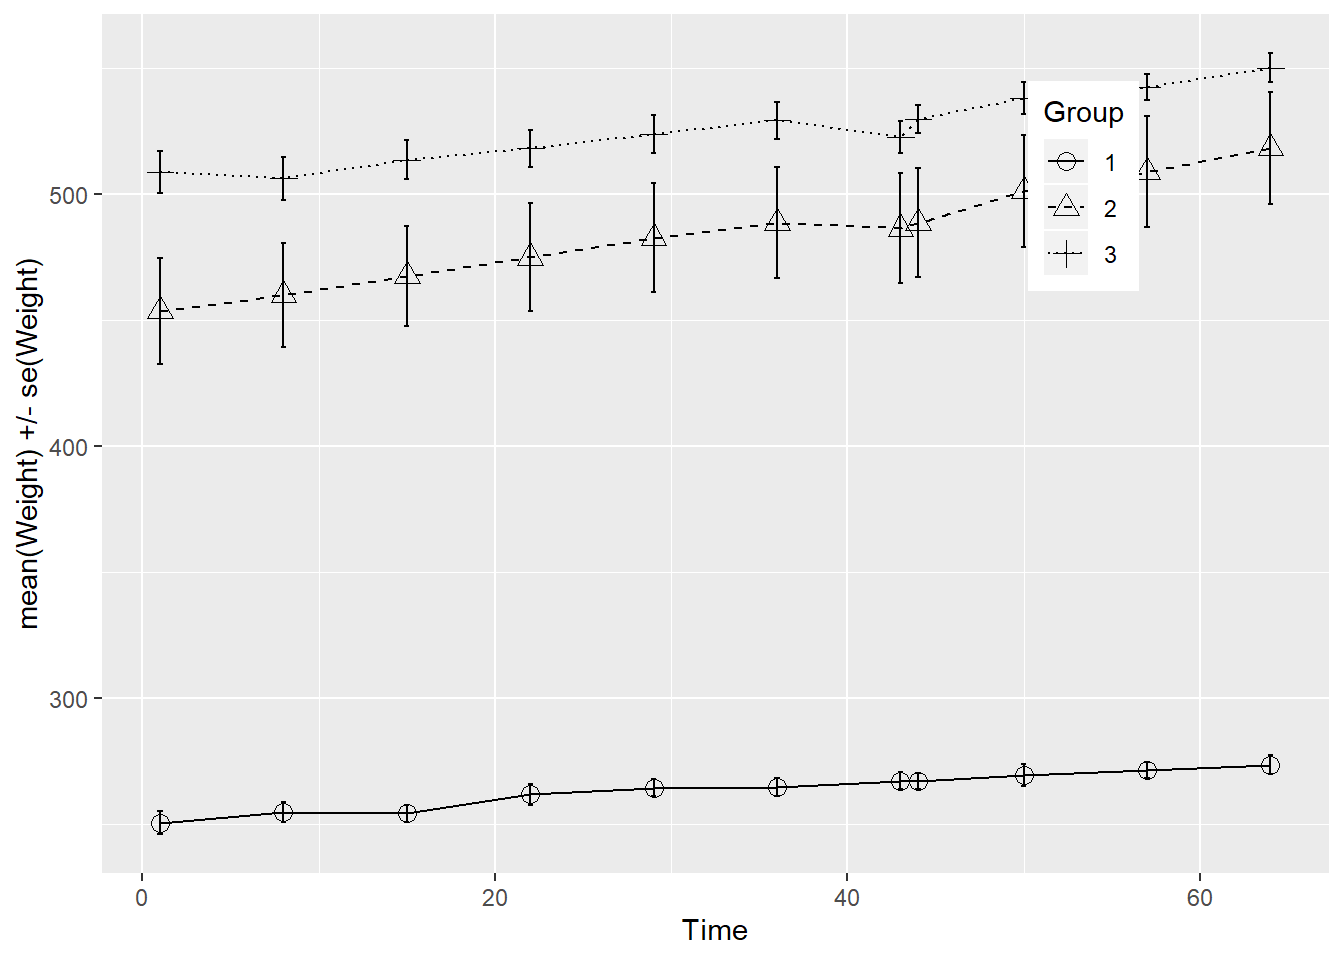
\includegraphics{jyt_chapter10_files/figure-latex/unnamed-chunk-6-1.pdf}

\hypertarget{instructions-3}{%
\subsubsection{Instructions}\label{instructions-3}}

\begin{itemize}
\tightlist
\item
  Adjust the code: replace both \texttt{1}s and give the \texttt{lm()}
  function a formula where points is explained by attitude. Adjust the
  data argument to use the learning2014 data.frame
\item
  Use \texttt{summary()} to look at a summary of the fitted model.
\end{itemize}

\hypertarget{r-code-3}{%
\subsubsection{R code}\label{r-code-3}}

\begin{Shaded}
\begin{Highlighting}[]
\CommentTok{# Work with the exercise in this chunk, step-by-step. Fix the R code!}

\CommentTok{# learning2014 is available}

\CommentTok{# Explain students statistics exam points with their attitude toward statistics using a linear model}

\CommentTok{# Create object my_fit explaining points with attitude in the learning2014 data}
\NormalTok{my_fit <-}\StringTok{ }\KeywordTok{lm}\NormalTok{(}\DecValTok{1} \OperatorTok{~}\StringTok{ }\DecValTok{1}\NormalTok{, }\DataTypeTok{data =} \OtherTok{NULL}\NormalTok{) }\CommentTok{#??? #??? #???}

\CommentTok{# Look at a summary of my_fit}
\CommentTok{#???}
\end{Highlighting}
\end{Shaded}

\hypertarget{interpreting-a-fitted-model}{%
\subsection{10.5 Interpreting a fitted
model}\label{interpreting-a-fitted-model}}

Now that we have estimated the parameters of our (simple) model, it is
time to interpret the results! The focus is mainly on the regression
coefficients and their p-values. Find the instructions of interpreting
these (from a suitable web resource, for example).

Type \texttt{summary(my\_fit)} on the R console. Which of the following
choices is correct?

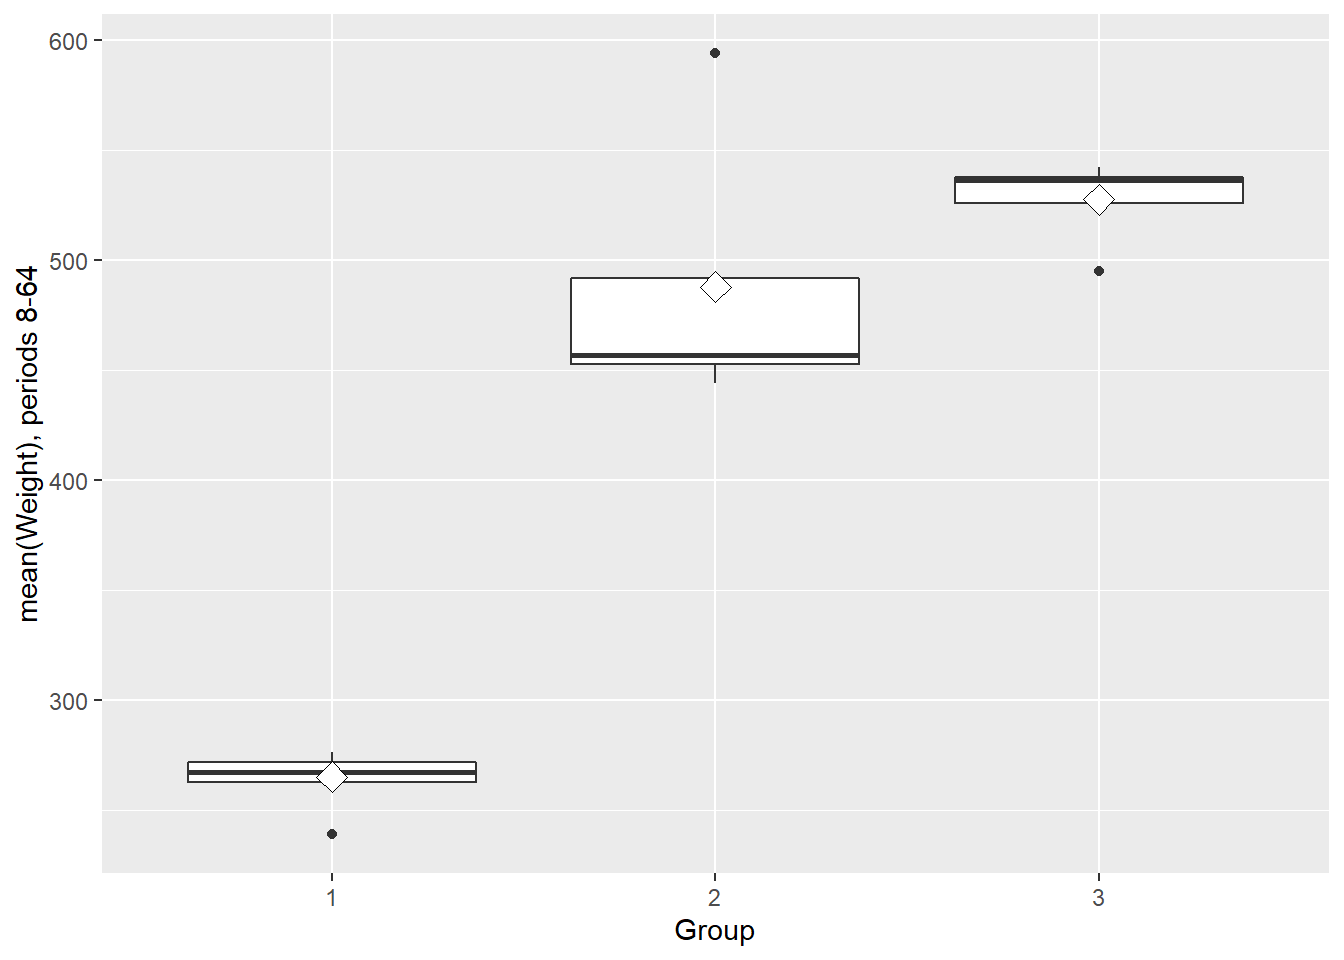
\includegraphics{jyt_chapter10_files/figure-latex/unnamed-chunk-8-1.pdf}

\hypertarget{instructions-4}{%
\subsubsection{Instructions}\label{instructions-4}}

\begin{itemize}
\tightlist
\item
  When a students attitude increases by one unit, the expected increase
  of exam points is 11.6 units. The effect is statistically significant.
\item
  When a students attitude increases by one unit, the expected decrease
  of exam points is 3.5 units. The effect is statistically significant.
\item
  When a students attitude increases by one unit, the average increase
  of exam points is 3.5 units. The effect is statistically significant.
\item
  When a students attitude increases by one unit, the expected increase
  of exam points is 3.5 units. The effect is not statistically
  significant.
\end{itemize}

Which choice is correct? Copy it below:

\begin{itemize}
\tightlist
\item
  ???
\end{itemize}

\hypertarget{checking-the-validity-of-model-assumptions}{%
\subsection{10.6 Checking the validity of model
assumptions}\label{checking-the-validity-of-model-assumptions}}

Let us now return to the assumptions of our model. We started by looking
at the plausibility of a linear relationship, which was the first
assumption. We have two assumptions left unchecked:

\begin{enumerate}
\def\labelenumi{\arabic{enumi}.}
\tightlist
\item
  \textbf{The variability in (prediction) errors is constant over
  possible values of the explanatory variable(s)}
\item
  \textbf{The (prediction) errors are normally distributed}
\end{enumerate}

The former can be studied graphically by plotting the predictions
(fitted values) of our model against the prediction errors (residuals).
If there is a visible pattern, that would mean a likely violation to the
constant variability assumption.

Also the latter assumption can be studied graphically. A q-q plot is a
powerful way to check if observations follow a theoretical distribution.
If this is the case, then the quantile points in the q-q plot should
approximately follow a straight increasing line. Deviations from the
normality assumption should show a clear non-linear pattern.

When a linear model object such as \texttt{my\_fit} is given to the
\texttt{plot()} function as the first argument, \texttt{plot()} draws
multiple diagnostic plots related to the model. Type
\texttt{plot(my\_fit)} on the R console and choose the correct answer.

\hypertarget{instructions-5}{%
\subsubsection{Instructions}\label{instructions-5}}

\begin{itemize}
\tightlist
\item
  The scatter plot of fitted values and residuals shows that the values
  of the residuals depend on the fitted values, violating assumption 1.
  The q-q plot shows that the distribution of the residuals is
  approximately normal.
\item
  The scatter plot of fitted values and residuals shows that the values
  of the residuals do not depend on the fitted values. The q-q plot
  shows that the residuals and fitted values are independent.
\item
  The scatter plot of fitted values and residuals shows that the values
  of the residuals do not depend on the fitted values. The q-q plot
  shows that the distribution of the residuals is approximately normal.
\item
  The scatter plot of fitted values and residuals shows that the values
  of the residuals do not depend on the fitted values. The q-q plot
  shows that the distribution of the residuals is not approximately
  normal, violating assumption 2.
\end{itemize}

Which choice is correct? Copy it below:

\begin{itemize}
\tightlist
\item
  ???
\end{itemize}

Great work! You are really learning the linear models.

\hypertarget{making-predictions-based-on-the-model}{%
\subsection{10.7 Making predictions based on the
model}\label{making-predictions-based-on-the-model}}

Okey, so we have a linear model which seems to fit our standards. What
can we do with it?

The model quantifies the relationship between the explanatory
variable(s) (attitude) and the dependent variable (points). The model
can also be used for predicting the dependent variable based on new
observations of the explanatory variable(s).

\hypertarget{instructions-6}{%
\subsubsection{Instructions}\label{instructions-6}}

\begin{itemize}
\tightlist
\item
  Create object \texttt{my\_fit} and \texttt{new\_attitudes}
\item
  Adjust the code: Replace \texttt{NULL} with the new attitudes to
  create a new data frame with an attitude column
\item
  Print out the new data frame
\item
  Use the \texttt{predict()} function to predict the new students exam
  points based on their attitude. The argument \texttt{newdata} should
  be a data.frame with the new observations for the explanatory
  variable(s).
\end{itemize}

\hypertarget{r-code-4}{%
\subsubsection{R code}\label{r-code-4}}

\begin{Shaded}
\begin{Highlighting}[]
\CommentTok{# Work with the exercise in this chunk, step-by-step. Fix the R code!}

\CommentTok{# learning2014 is available}

\CommentTok{# Create object my_fit explaining students exam points with attitude towards statistics}
\NormalTok{my_fit <-}\StringTok{ }\KeywordTok{lm}\NormalTok{(points }\OperatorTok{~}\StringTok{ }\NormalTok{attitude, }\DataTypeTok{data =}\NormalTok{ learning2014)}

\CommentTok{# New observations}
\NormalTok{new_attitudes <-}\StringTok{ }\KeywordTok{c}\NormalTok{(}\StringTok{"Miia"}\NormalTok{ =}\StringTok{ }\FloatTok{3.8}\NormalTok{, }\StringTok{"Matti"}\NormalTok{=}\StringTok{ }\FloatTok{4.4}\NormalTok{, }\StringTok{"Riikka"}\NormalTok{ =}\StringTok{ }\FloatTok{2.2}\NormalTok{, }\StringTok{"Pekka"}\NormalTok{ =}\StringTok{ }\FloatTok{2.9}\NormalTok{)}
\NormalTok{new_data <-}\StringTok{ }\KeywordTok{data.frame}\NormalTok{(}\DataTypeTok{attitude =} \OtherTok{NULL}\NormalTok{) }\CommentTok{#???}

\CommentTok{# Print out the new data}
\CommentTok{#???}

\CommentTok{# Predict the new students exam points based on attitude}
\KeywordTok{predict}\NormalTok{(my_fit, }\DataTypeTok{newdata =} \OtherTok{NULL}\NormalTok{) }\CommentTok{#???}
\end{Highlighting}
\end{Shaded}

\begin{verbatim}
##        1        2        4        5        6        7        8        9 
## 18.33553 25.03390 18.33553 20.45080 25.73899 23.97626 24.68136 23.97626 
##       11       12       13       14       15       16       17       18 
## 24.68136 22.91863 24.68136 23.97626 23.97626 23.62372 23.27117 19.04062 
##       20       21       22       24       26       27       28       29 
## 21.50844 27.50172 20.45080 22.21353 26.09154 26.09154 22.56608 23.97626 
##       30       32       33       34       35       36       37       38 
## 20.09826 23.27117 22.91863 22.91863 17.63044 23.27117 20.80335 22.91863 
##       39       40       41       42       44       45       47       48 
## 21.15590 25.03390 22.91863 20.80335 25.38645 25.03390 18.68807 24.68136 
##       49       50       51       52       53       54       55       56 
## 23.27117 22.56608 20.45080 26.09154 25.73899 20.45080 23.27117 21.15590 
##       57       58       60       61       62       63       64       65 
## 24.68136 21.15590 24.68136 22.21353 20.09826 22.21353 18.33553 26.44409 
##       66       68       69       70       71       72       73       74 
## 20.09826 20.80335 22.21353 22.56608 18.68807 18.33553 21.50844 21.86099 
##       75       76       77       78       79       80       81       82 
## 21.50844 18.68807 26.44409 21.15590 23.97626 23.97626 25.03390 26.44409 
##       83       84       85       86       87       88       89       90 
## 24.32881 24.32881 24.32881 24.68136 22.56608 25.03390 26.44409 19.04062 
##       91       92       93       94       95       96       97       99 
## 23.62372 20.45080 22.91863 23.27117 21.86099 19.04062 22.91863 19.74571 
##      100      102      103      104      105      106      107      108 
## 26.09154 28.20682 22.21353 20.09826 25.73899 23.62372 18.33553 29.26445 
##      109      110      111      112      113      114      115      116 
## 17.63044 28.20682 22.56608 23.62372 22.56608 22.56608 20.45080 24.32881 
##      117      118      119      120      121      122      123      124 
## 23.27117 17.98298 25.38645 20.09826 24.68136 26.09154 17.63044 20.80335 
##      126      127      128      129      131      132      133      134 
## 22.91863 25.03390 23.97626 23.27117 22.91863 23.27117 19.74571 19.74571 
##      135      136      137      138      139      140      141      142 
## 23.62372 25.03390 20.80335 25.38645 24.68136 27.14918 21.15590 21.50844 
##      144      145      147      148      149      150      151      152 
## 22.56608 17.27789 25.38645 19.04062 21.50844 26.09154 22.91863 16.57280 
##      153      154      155      156      157      158      159      161 
## 28.55936 20.45080 19.74571 20.45080 20.80335 23.97626 25.03390 27.14918 
##      162      163      164      165      166      167      168      169 
## 18.68807 21.86099 25.73899 21.86099 19.74571 21.86099 21.50844 25.38645 
##      170      171      172      173      174      175      176      177 
## 21.86099 24.32881 24.68136 23.97626 23.27117 24.32881 20.80335 22.91863 
##      178      179      180      181      182      183 
## 19.04062 22.56608 21.86099 22.91863 25.38645 21.86099
\end{verbatim}

Awesome work! That was it! Thank you so much for participating in the
course!

Please continue learning more R in the future. I predict that it will be
beneficial to you!


\end{document}
